\documentclass[11pt]{article}

\usepackage[a4paper,margin=2.5cm]{geometry}
\usepackage{graphicx}
\usepackage{float}
\usepackage{booktabs}

\title{HPC: Labwork \#5}
\author{Nguyen Trong Minh}
\date{Friday, October 2, 2026 \\ SonTG}

\begin{document}

\maketitle

\section{Implementation}

The goal of this labwork is to blur an image with a Gaussian filter on the GPU, once without shared memory and once with shared memory, and compare the two. First I convert the image to grayscale with the 2D kernel from labwork 4. Because the three channels of a gray image are the same, I only blur channel 0 and write the result back to all three channels, so each thread does the work once instead of three times.

\subsection{Gaussian kernel}

I use a 7-tap Gaussian kernel $[1, 6, 15, 20, 15, 6, 1] / 64$. The Gaussian blur is separable, so instead of doing a full $7 \times 7$ convolution, I blur every row with the 1D kernel first, then blur every column of that result with the same 1D kernel\footnote{\texttt{https://medium.com/@RaymondTayBL/gaussian-blur-separable-convolution-vs-full-2d-convolution-d5e9b64bf84f}}. This gives the same result but each pixel only needs $7 + 7 = 14$ multiplications instead of $49$. For one pixel, the row pass is:

\[
    \mathrm{out}[y, x] = \sum_{i=0}^{6} k[i] \cdot \mathrm{img}[y,\ x - 3 + i].
\]

The 3 here is the radius of the kernel: each pixel looks at 3 neighbours on the left and 3 on the right. Near the border of the image, $x - 3 + i$ can go outside the image, so I clamp it into $[0, \mathrm{width} - 1]$, which means the edge pixel is repeated.

The column pass reads from the output of the row pass and writes into a different array. It cannot write back into the same array, because blocks run in any order and one block could overwrite pixels that another block still needs to read.

\subsection{Without shared memory}

This version is simple. Each thread gets its pixel $(x, y)$ from \texttt{cuda.grid(2)}, reads its 7 neighbours directly from global memory with the formula above, and writes the sum. I wrote one kernel for the row pass and one for the column pass, the only difference is which index moves.

\subsection{With shared memory}

In the version without shared memory, neighbouring threads read almost the same pixels, so each input pixel is read from global memory 7 times. The idea of shared memory is that a block copies the pixels it needs into a small and fast memory once, then all threads in the block read from there.

I use blocks of $8 \times 8$ threads. For the row pass, a block outputs 8 pixels per row, but the pixels at the left and right edge of the block still need 3 neighbours that belong to the next block. These extra pixels are called the halo. So the shared array of the block has $8 + 2 \times 3 = 14$ columns and 8 rows, shape $8 \times 14$. The kernel works in 3 steps:

\begin{enumerate}
    \item \textbf{Load.} Every thread copies its own pixel into the tile at column \texttt{tx + 3}, because the first 3 columns are kept for the left halo. Then the first 3 threads (\texttt{tx < 3}) also load the pixel 3 columns to their left into column \texttt{tx}, and the last 3 threads (\texttt{tx >= 5}) load the pixel 3 columns to their right into column \texttt{tx + 6}. To check the index, thread 0 must fill column 0 and thread 7 must fill column 13.
    \item \textbf{Wait.} \texttt{cuda.syncthreads()} makes all threads in the block wait until the whole tile is loaded. Without it, a thread could read a slot that another thread has not written yet. The bounds check comes after this line, because if some threads return early they never reach the barrier.
    \item \textbf{Compute.} The neighbour $i$ of a thread is at tile column $(tx + 3) - 3 + i = tx + i$, so the sum just reads \texttt{sm[ty, tx + i]} for $i = 0 \dots 6$.
\end{enumerate}

The column pass is the same with rows and columns swapped: the tile is $14 \times 8$ and the halo is above and below. I had to write it as a separate kernel, because the shape of a shared array must be fixed when Numba compiles the kernel, so one kernel cannot have both shapes.

The mistakes I made while writing this were: forgetting to load the tile at all (shared memory starts with garbage), putting the right halo at \texttt{tx - 3} instead of \texttt{tx + 6} (which overwrote the centre pixels of other threads), and calling \texttt{cuda.synchronize()} inside the kernel instead of \texttt{cuda.syncthreads()}. The first one is for the CPU to wait for the GPU, the second one is for threads in a block to wait for each other.

\subsection{CPU version and timing}

To compare with the CPU, I wrote the same row and column blur as normal loops and compiled them with Numba \texttt{njit}, once on a single core and once with \texttt{parallel=True}, where the loop over rows is split across 8 CPU threads with \texttt{prange}. Unlike labwork 3 and 4, the CPU code is compiled and not a Python loop, so the comparison is fairer.

The image is resized to $512 \times 512$. The grayscale step is not timed, only the two blur passes are. Every version is run once to warm up first, because the first call includes the JIT compilation, and then 20 times, and I take the average. For the GPU I call \texttt{cuda.synchronize()} before and after the timed runs, because kernel launches are asynchronous.

\section{Output Images}

All four versions produce the same image. The program checks this with \texttt{np.allclose}, and the saved GPU and CPU images are the same pixel by pixel.

\begin{figure}[H]
    \centering
    \begin{minipage}[t]{0.48\textwidth}
        \centering
        
\includegraphics[width=\linewidth]{blurred_grey_cpu.png}
        \small CPU output
    \end{minipage}
    \hfill
    \begin{minipage}[t]{0.48\textwidth}
        \centering
        
\includegraphics[width=\linewidth]{blurred_grey.png}
        \small GPU output (shared memory)
    \end{minipage}
    \caption{Blurred grayscale images generated by the CPU and CUDA implementations.}
    \label{fig:outputs}
\end{figure}

The blur is quite light. This 7-tap kernel is close to a Gaussian with $\sigma \approx 1.2$ pixels, so it only softens small details. A stronger blur needs a bigger $\sigma$, and the radius of the kernel has to grow to about $3\sigma$.

\section{Result}

The result is shown in Table~\ref{tab:timing} and Figure~\ref{fig:timing}. The speedup is compared with the CPU single core version.

\begin{table}[H]
    \centering
    \begin{tabular}{lcc}
        \toprule
        Version & Execution time (ms) & Speedup \\
        \midrule
        CPU single core           & 2.369 & $\times 1.0$ \\
        CPU multi-thread (8 threads) & 0.633 & $\times 3.7$ \\
        GPU global memory         & 0.234 & $\times 10.1$ \\
        GPU shared memory         & 0.233 & $\times 10.2$ \\
        \bottomrule
    \end{tabular}
    \caption{Average execution time of the separable 7-tap Gaussian blur (row pass + column pass) on a $512 \times 512$ image, mean of 20 runs.}
    \label{tab:timing}
\end{table}

\begin{figure}[H]
    \centering
    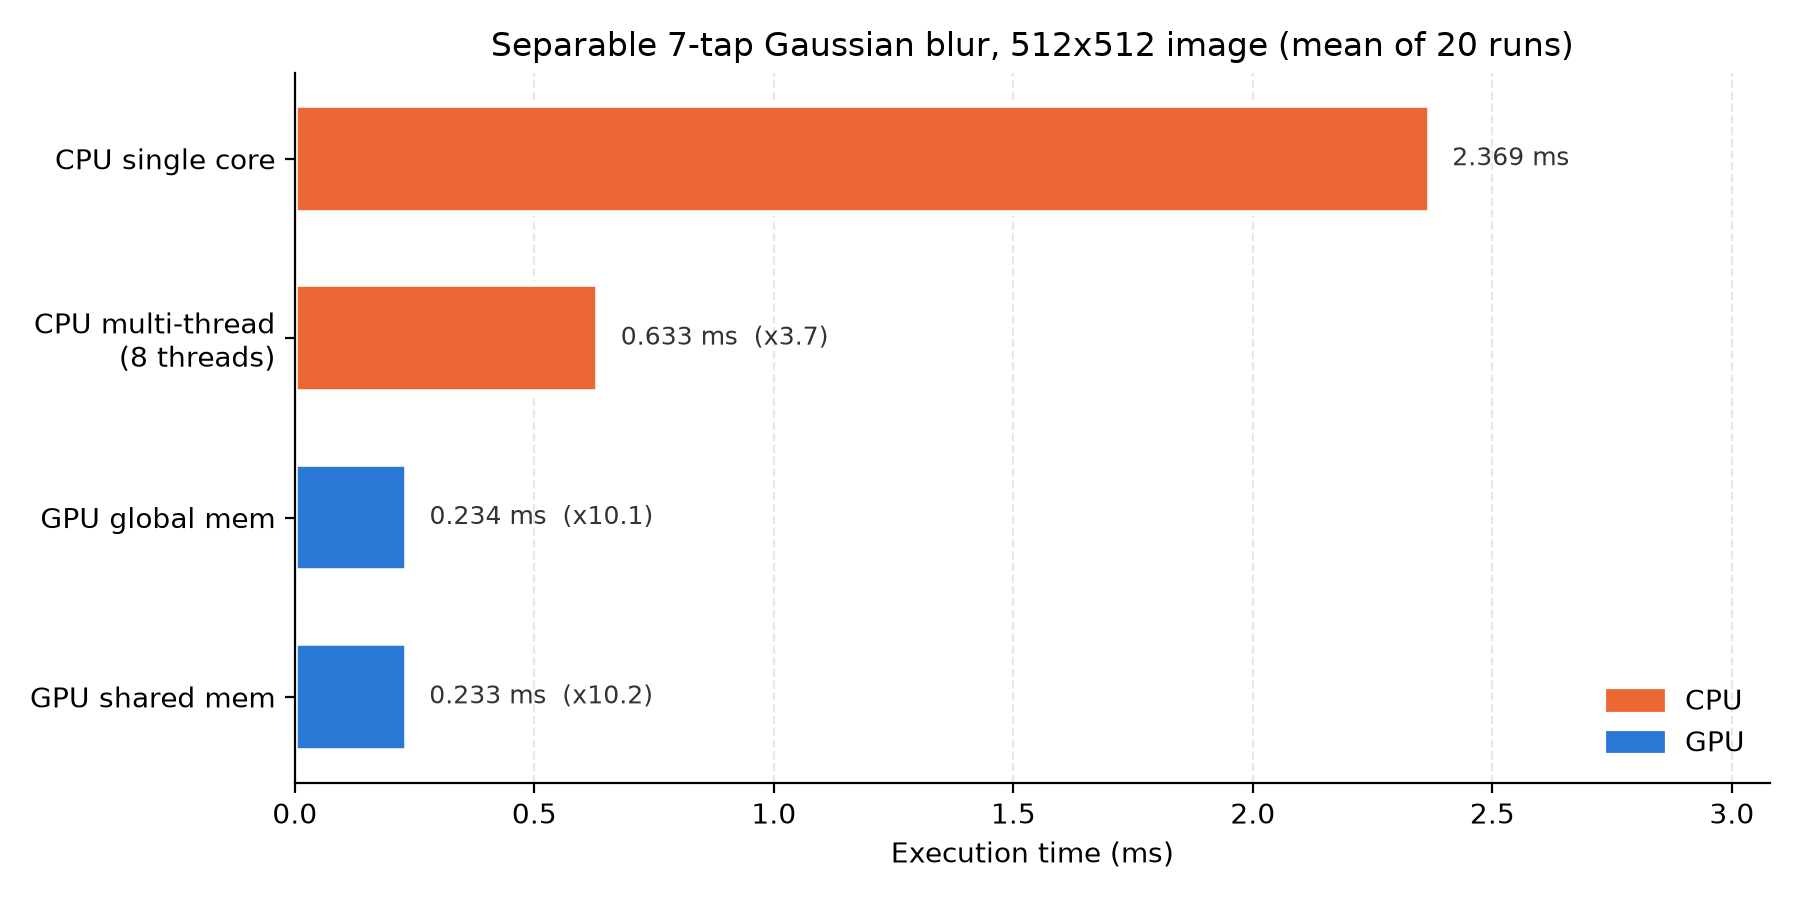
\includegraphics[width=\textwidth]{execution_time.png}
    \caption{Execution time of the CPU and GPU versions.}
    \label{fig:timing}
\end{figure}

The surprising part is that shared memory does not make the blur faster. The two GPU versions take 0.234 and 0.233 ms, which is less than 1\% difference, so it is just noise. I think there are a few reasons:

\begin{itemize}
    \item The kernel is small. Each pixel only reads 7 neighbours, so there is not much repeated reading to save.
    \item Modern GPUs have an L1 cache. When neighbouring threads read the same pixels from global memory, most of the reads are already served from the cache, so the global memory version gets part of the benefit of shared memory for free.
    \item The shared memory version has extra work: loading the halo and waiting at \texttt{syncthreads()}. With $8 \times 8$ blocks the halo is large compared to the block, each block loads 14 pixels per row to output only 8.
    \item The image is small ($512 \times 512 = 262{,}144$ pixels), so the GPU is not very busy, and fixed costs like launching the two kernels take a bigger part of the time.
\end{itemize}

I expect shared memory to matter more with a bigger kernel, for example $\sigma = 5$ needs a radius of 15, so each pixel reads 31 neighbours instead of 7. For that, the halo loading has to be changed, because with $8 \times 8$ blocks only 8 threads are available to load a halo of 15 pixels on each side.

Compared with the CPU, the GPU is about 10 times faster than one core and about 2.7 times faster than 8 threads. This speedup is much smaller than the 3,000 times in labwork 3 and 4, because the CPU code is now compiled with Numba instead of running as a Python loop. Using 8 threads on the CPU only gives $\times 3.7$ instead of $\times 8$, I think because the work is very short (around 2 ms) so the cost of starting and synchronizing the threads is not small compared to the work itself.

\section{Conclusion}

All versions produce the same blurred image, and the GPU is about 10 times faster than a compiled single core CPU version. For this 7-tap blur, shared memory gives no speedup over reading directly from global memory, because the kernel is small and the L1 cache already handles most of the repeated reads. The main things I learned in this labwork are how shared memory works: it belongs to one block, it has to be filled by the threads themselves, it needs \texttt{cuda.syncthreads()} before other threads read from it, and its shape has to be fixed at compile time. I also learned that the halo is the hardest part, because a small mistake in the index silently overwrites other threads' data instead of giving an error.

\end{document}
